\subsection{Modeling Circuits with Polynomial Ideals}\label{sec:pmodel} 

% Rectification begins after verification detects the presence of bugs
% in the design. 
% For verification of finite field arithmetic circuits,
% the approach based on \cite{lv:tcad2013} has been shown to be 
% successful. As the algebraic setup for verification is augmented
% for subsequent rectification, we review the main concepts from
% \cite{lv:tcad2013} below. 
% The algebraic setup used in our MFR checking procedure 
% We perform verification using the approach presented in~\cite{lv:tcad2013}. 
% , utilize the same setup as a starting point for MFR checking. 
% We review the main concepts from~\cite{lv:tcad2013} below:

% We use an augmentation of the algebraic setup presented in~\cite{lv:tcad2013}
% as a starting point for the MFR checking procedure. We therefore review the 
% main concepts and verification setup from~\cite{lv:tcad2013} below:

A multivariate polynomial $f$ over $\Fkn$ is given as a \spec,
where $n$ is the operand word-length (data-path size). A %corresponding
combinational circuit $C$ is given as its (faulty) implementation. 
The function implemented by $C$ is modeled with a system of
polynomials over $R=\Fkn[Z,A,X]$, where $X = \{x_1, \dots,
x_d\}$ corresponds to all the bit-level variables (nets) in the
circuit. Let $X_{PO} \subset X$, and $X_{PI} \subset X$ denote the set of all primary 
output variables, and primary input variables from $C$, respectively. 
Further, $Z=\{z_0,\dots,z_{n-1}\}$ and $A = \{a_0,\dots,a_{n-1}\}$
represent the output and input operand words of the circuit, respectively,
where $z_i\in X_{PO}$ and $a_i\in X_{PI}$. 
% The field $\Fkn$ is constructed as $\Fkn = \Ftwo[x]\pmod{P_n(x)}$, where
% $P_n(x)$ is the given primitive polynomial of degree $n$
% with $\ga$ as a root, i.e. $P_n(\ga) =0$. 
As $C$ comprises Boolean logic gates, the gates are represented by
polynomials $\pmod{2}$, i.e. over $\F_2 (\subset \Fkn)$, using the
mapping $\B\mapsto \F_2$:
% as follows: 

\begin{small} 
\begin{align}
\label{bool2poly}
\begin{split}
z =  \neg a \mapsto z+a+1;& ~~~\hspace{0.2in} z =  a \wedge b \mapsto z+a \cdot b;\\
z =  a \vee b \mapsto z+a+b+a \cdot b;& ~~~\hspace{0.2in} z =  a \oplus b \mapsto z+a+b;
\end{split}
\end{align}
% \vspace{-0.15 in}
\end{small}

% \begin{small} 
% \begin{equation}
% \label{bool2poly}
% \begin{split}
% z =  \neg a &\rightarrow z+a+1 \pmod 2  \\
% z =  a \wedge b &\rightarrow z+a \cdot b \pmod 2\\
% z =  a \vee b &\rightarrow z+a+b+a \cdot b \pmod 2 \\
% z =  a \oplus b &\rightarrow z+a+b \pmod 2 
% \end{split}
% \end{equation}
% \end{small}
% \vspace{-0.15in}

Algebraically, the correspondences between the bit-level and word-level
variables of the circuit are represented as:
% \vspace{-0.08in}
\begin{equation}
\label{ip-word-level}
\begin{split}
 f_1: Z =  z_0 +\gamma \cdot  z_1 + \dots +\gamma^{n-1} \cdot z_{n-1},\\
 f_2: A =  a_0 +\gamma \cdot a_1 + \dots +\gamma^{n-1} \cdot a_{n-1},
\end{split}
\end{equation}
where $P_n(\ga) =0$. Since $\F_2 \subset \Fkn$, the polynomials in 
Eqn. (\ref{bool2poly}) can also be interpreted as polynomials over $\Fkn$. 
% The advantage of working over $\Fkn$ is that we can represent and manipulate 
% both the bit-level and $n$-bit word-level polynomials in one unified domain, $\Fkn$.
Thus, the circuit is represented by a set of polynomials
$F=\{f_1,\dots,f_s\} \subset R$. Let $J =\langle F\rangle$ be the
ideal generated by this set.
%Let $X_{PI} \subset \{x_1,\dots,x_d\}$ be the primary input variables
%of the circuit. Let $F_0^{PI}=\{x_i^2-x_i:x_i\in X_{PI}\}$ denote the
%set of bit-level vanishing polynomials in primary inputs, and let $J_0
%= \langle F_0^{PI} \rangle$ be the ideal of vanishing polynomials.
Let $F_0 = \{x_i^2-x_i, Y^{2^n}-Y~|~x_i \in$ bit-level variables,
$Y \in$ word-level variables$\}$ be the set of all vanishing
polynomials, and $J_0 = \langle F_0\rangle$ the corresponding ideal.
% of all bit- and word-level vanishing polynomials. 
% It is shown in \cite{lv:phd} that it is 
% sufficient to include vanishing polynomials for only the primary input
% bits $X_{PI}$ in $J_0$, represented as $\jzxpi$. This ensures that the nets in the circuit can
% only assume values in $\F_2$, and the variables $Y$ only assume values in
% $\Fkn$. For simplicity, it is assumed from hereon that $J_0 = \langle F_0\rangle$ 
% represents $\jzxpi$, unless specified otherwise.
Then, ideal $J+J_0 = \langle F \cup F_0\rangle$ models the functionality of
$\impl ~C$. 

One can verify the correctness of the circuit $C$ by checking
if the given $\spec$ is implied by the ideal representing 
$C$. In other words, $f \equiv C \iff f\xrightarrow{GB(J+J_0)}_+0$
\cite{lv:tcad2013}. 
% Using a set ($F$) of polynomials to describe
% the logic circuit, along with a set of vanishing 
% polynomials ($F_0$) over the field $\Fkn$, the 16
% verification problem was formulated as a (radical) ideal membership test, requiring a
% \Grobner basis. Drawing inspirations from [128], the authors in [83] also exploited the
% same concept of deriving a specialized term order > to simplify the ideal membership
% test. In particular, it was shown that > could be derived by performing a reverse topological
% traversal on the circuit. Imposition of this term order > rendered the set of polynomials
% itself a \Grobner basis, and verification was then performed simply by a GB-reduction.
% Obviating the need of GB computation while moving the complexity of verification to
% polynomial divisions,
% While it is assumed that the given circuit $C$ is buggy, it is important 
% to note that the verification test can be formulated as {\textit{ideal
% membership  testing}} of $f$ in $J+J_0$ using
% GB~\cite{lv:tcad2013}, i.e. by  
% checking if $f\xrightarrow{GB(J+J_0)}_+0$.
% It has now become standard practice to impose {\it Reverse Topological Term Order (RTTO)} to 
% overcome the complexity of GB computations, which ensures the set of
% polynomials $F\cup F_0$ itself constitute a GB of $J+J_0$. This simplifies
% the above {\textit{ideal membership testing}} to that of checking if the polynomial division
% $f\xrightarrow{F+F_{0}}_+0$.
% . When $C$ correctly implements $f$, then $f$ agrees
% with every evaluation of all the nets in $C$. In other words, $f$
% vanishes on $V(J)$, or equivalently $f \in I(V(J))$. The Strong
% Nullstellensatz in finite fields (Thm. \ref{thm:strong-ns}) tells us
% %Nullstellensatz in finite fields tells us
% that $I(V(J)) = J + J_0$, where $J_0 = \langle F_0 \rangle = \langle x_1^2-x_1,\dots
% ,x_d^2-x_d,Z^{2^n}-Z, A^{2^n}-A\rangle$. Thus, the verification test can be formulated as
% ideal membership testing of $f$ in $J+J_0$ using \Grobner bases: We will
% check if $f\xrightarrow{GB(J+J_0)}_+0$?
% Further, the authors~\cite{lv:tcad2013} impose a specialized term order
% '$>$` called the {\it Reverse Topological Term Order (RTTO)} on the
% polynomials. RTTO is derived by ordering the nets (variables) of $C$
% in reverse topological order from primary outputs to primary inputs,
% and imposing a {\it lex} order on the monomials. It has
% now become standard practice to utilize RTTO-style term orders to 
% overcome the complexity of GB computations.
% RTTO $>$ ensures
% that each net at a gates output appears as a leading term of some
% polynomial in $F$. 
% As each gate output is a distinct net, the
% leading terms of all polynomials in $F$ become relatively
% prime. Thm. 6.1 and Cor. 6.1 in \cite{lv:tcad2013} show that due to
% the above characteristics, {\it RTTO $>$ renders the set of
%   polynomials $F\cup F_0$ itself a GB of $J+J_0$.}
%As the set $F\cup F_0$ is a GB is itself,
% As a result, the expensive GB computation is avoided altogether, and
% the verification check reduces to that of polynomial division
% $f\xrightarrow{F,F_{0}}_+r$, and checking whether $r=0$.
In the manuscript, we use the circuit of Fig. \ref{fig:mas_bug_W},
which is borrowed from \cite{Vkrao:ISQED21}, as a running example to
demonstrate our algebraic approach for MFR.  




\begin{Example}
\label{verify_ex}
{\it 
The circuit $C$ in Fig. \ref{fig:mas_bug_W} is a faulty
implementation of a 3-bit ($n$=3) Mastrovito multiplier. 
The field $\F_{2^3}$ is constructed using $P_3(x)=x^3+x+1$
with $\ga$ as a root, i.e. $P_3(\ga)=0$. The \spec
~polynomial is $f: Z + A\cdot B$, where $Z$ is the output word, and
$A,B$ the input words. Impose RTTO $>$ on the polynomials, i.e. a {\it
  lex term order} on all polynomials with the variables of $C$ ordered
reverse topologically from POs to PIs:
\begin{small}
% $\{Z\}>\{A>B\}>\{z_0>z_1>z_2\}>\{d_0>f_0>e_2>e_3\}>\{e_0>e_1>rr_0>d_6>d_7>d_8\}>\{d_1>d_2>d_3>r_0>d_5>rr_1\}>\{r_1>rr_3>rr_2\}>\{r_2>r_3>rr_4\}>\{r_4>d_4\}>\{a_0>a_1>a_2>b_0>b_1>b_2\}$
$\{Z\}>\{A>B\}>\{z_0>z_1>z_2\}>\cdots>\{d_1>d_2>d_3>r_0>d_5>rr_1\}>\{r_1>rr_3>rr_2\}>\{r_2>r_3>rr_4\}>\{r_4>d_4\}>\{a_0>a_1>a_2>b_0>b_1>b_2\}$.
\end{small}

Under RTTO $>$, the following
polynomials represent $C$: 
%the function implemented by $C$,
%with terms ordered according to RTTO $>$.
% {\small\begin{flalign*}
% f_1:Z + z_0 +\ga z_1 + \ga^2 z_2;     &\quad f_{16}:d_8 + a_2b_0; \\
% f_2:A + a_0 +\ga a_1 + \ga^2 a_2;     &\quad f_{17}:d_1 + a_1b_0; \\
% f_3:B + b_0 +\ga b_1 + \ga^2 b_2;     &\quad f_{18}:d_2 + a_0b_1; \\
% f_4:z_0 + d_0 + e_1;                  &\quad f_{19}:d_3 + a_1b_2; \\
% f_5:z_1 + f_0 + rr_0;                 &\quad f_{20}:r_0 + r_1d_4; \\
% f_6:z_2 + e_2 + e_3;              &\quad f_{21}:d_5 + a_2b_2; \\
% f_7:d_0 + a_0b_0;                     &\quad f_{22}:rr_1 + rr_2+rr_3; \\
% f_8:f_0 + e_0 + e_1;                  &\quad f_{23}:r_1 + r_2+r_3; \\
% f_9:e_2 + rr_0 + d_6;                 &\quad f_{24}:rr_2 + b_2 + 1; \\ 
% f_{10}:e_3 + d_7 + d_8;               &\quad f_{25}:r_2 + b_2 + 1; \\
% f_{11}:e_0 + d_1 + d_2;           &\quad \red{f_{26}:r_3 + d_4 + r_4;}\\
% f_{12}:e_1 + d_3 + r_0;               &\quad \red{f_{27}:rr_3 + rr_4 + b_2;} \\
% f_{13}:rr_0 + d_5rr_1;                &\quad f_{28}:d_4 + a_2b_1; \\
% f_{14}:d_6 + a_1b_1;              &\quad f_{29}:r_4 + a_2 + b_2 + a_2b_2; \\
% f_{15}:d_7 + a_0b_2;              &\quad f_{30}:rr_4 + a_2 + b_2 + a_2b_2; \\
% \end{flalign*}}
% \vspace{-0.13in}
% \begin{small}
% \begin{flalign*}
% f_1:Z + z_0 +\ga z_1 + \ga^2 z_2;     &\quad \dots\\
% f_2:A + a_0 +\ga a_1 + \ga^2 a_2;     &\quad f_{22}:rr_1 + rr_2+rr_3; \\
% f_3:B + b_0 +\ga b_1 + \ga^2 b_2;     &\quad f_{23}:r_1 + r_2+r_3; \\
% f_4:z_0 + d_0 + e_1;                  &\quad f_{24}:rr_2 + b_2 + 1; \\ 
% f_5:z_1 + f_0 + rr_0;                 &\quad f_{25}:r_2 + b_2 + 1; \\
% f_6:z_2 + e_2 + e_3;              &\quad \red{f_{26}:r_3 + d_4 + r_4;}\\
% f_7:d_0 + a_0b_0;                 &\quad \red{f_{27}:rr_3 + rr_4 + b_2;} \\
% f_8:f_0 + e_0 + e_1;              &\quad f_{28}:d_4 + a_2b_1; \\
% f_9:e_2 + rr_0 + d_6;                 &\quad f_{29}:r_4 + a_2 + b_2 + a_2b_2; \\
% \dots                             &\quad f_{30}:rr_4 + a_2 + b_2 + a_2b_2;
% \end{flalign*}
% \end{small}
\begin{small}
\begin{flalign*}
% \vspace{-0.12in}
f_1:Z + z_0 +\ga \cdot z_1 + \ga^2 \cdot z_2;   &\quad f_{22}:rr_1 + rr_3+rr_2; \\
f_2:A + a_0 +\ga \cdot a_1 + \ga^2 \cdot a_2;   &\quad f_{23}:r_1 + r_2+r_3;\\
f_3:B + b_0 +\ga \cdot b_1 + \ga^2 \cdot b_2;   &\quad \red{f_{26}:r_3 + r_4 + d_4;}\\
f_4:z_0 + d_0 + e_1;                &\quad {\red f_{27}:rr_3 + rr_4 + b_2;} \dots\\
\dots                               &\quad f_{30}:rr_4 + a_2+b_2+a_2b_2;
\end{flalign*}
\end{small}
% \vspace{-0.2in}
% \vspace{-0.1in}
% \begin{small}
% \begin{flalign*}
% f_1:Z + z_0 +\ga z_1 + \ga^2 z_2;   &\quad f_{22}:rr_1 + rr_2+rr_3; \\
% f_2:A + a_0 +\ga a_1 + \ga^2 a_2;   &\quad f_{23}:r_1 + r_2+r_3; \\
% f_3:B + b_0 +\ga b_1 + \ga^2 b_2;   &\quad \dots\\ 
% f_4:z_0 + d_0 + e_1;                &\quad \red{f_{26}:r_3 + d_4 + r_4;}\\
%                                     &\quad \red{f_{27}:rr_3 + rr_4 + b_2;} \\
%                                     &\quad \dots\\
% \dots                               &\quad f_{30}:rr_4 + a_2 + b_2 + a_2b_2;
% \end{flalign*}
% \end{small}
% The correct circuit will have polynomials $f_{10},f_{12},$ and $f_{18}$ above replaced by 
% $f_{10_c} = e_0 + d_1 + d_2, f_{12_c}:d_5 + a_2b_2,$ and  $f_{18_c}:d_2 + a_2b_1$ respectively.
where the polynomials $f_{26}, f_{27}$ correspond to the introduced
bugs. Then $F = \{f_1,\dots,f_{30}\}$, $F_0=\{a_0^2-a_0,\dots,z_2^2-z_2,A^8-A,B^8-B,Z^8-Z\}$. 
%under RTTO $>$, $F\cup F_{0}$ constitutes a GB of
So, ideal $J+J_0=\langle F\cup F_0\rangle$ encapsulates the function implemented by $C$. 
Computing $f: Z + A\cdot  B\xrightarrow{F,F_{0}}_+r$ results in $r =
 \ga^2(a_1a_2b_1b_2+a_1a_2b_2+a_2b_1b_2) +
 \ga^1(a_1a_2b_1b_2+a_1a_2b_2) + \ga^0(a_2b_1b_2)$. Since $r\neq 0$,
 the circuit is buggy.  
}
\end{Example}
% \vspace{-0.12in}

\begin{figure}[hbt]
    \begin{center}
    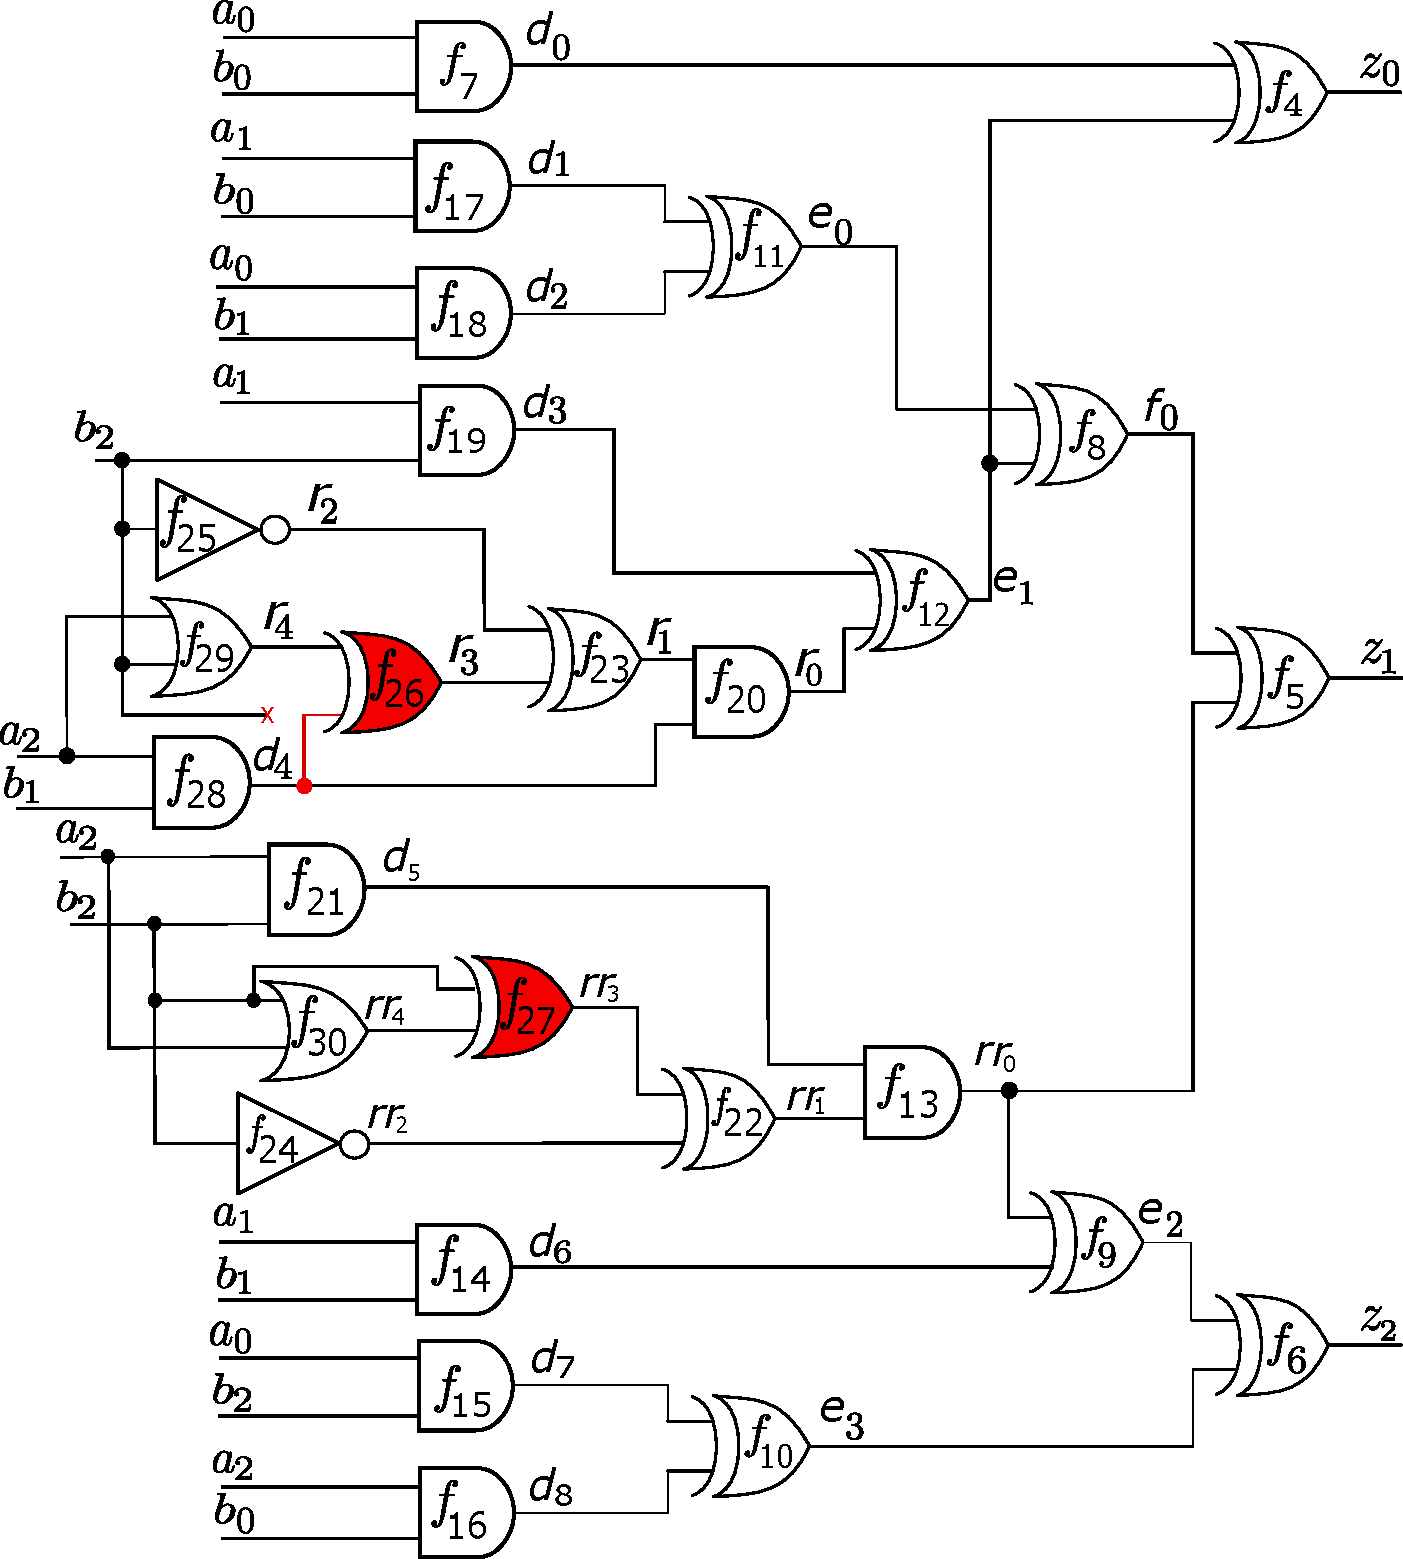
\includegraphics[scale = 0.29]{mas_3_ddc_mfr_a.pdf}
    \end{center}
    \Description{\caption{{\footnotesize  
        A faulty $\impl$ of the circuit $C$: a 3-bit finite
        field multiplier ($n$=3) with bugs introduced at net $r_3$
        (AND gate replaced with an XOR gate and one of the inputs
        mis-connected to $d_4$ instead of $b_2$) and net $rr_3$ (AND gate
        replaced with an XOR gate).}}}
    \caption{{\footnotesize  
        A faulty $\impl$ of the circuit $C$: a 3-bit finite
        field multiplier ($n$=3) with bugs introduced at net $r_3$
        (AND gate replaced with an XOR gate and one of the inputs
        mis-connected to $d_4$ instead of $b_2$) and net $rr_3$ (AND gate
        replaced with an XOR gate).}}  
    \label{fig:mas_bug_W}
    % \vspace{-0.25in}
\end{figure}
